\documentclass[10pt,twocolumn]{article}

\usepackage[margin=0.72in]{geometry}
\usepackage{amsmath,amssymb}
\usepackage{booktabs}
\usepackage{graphicx}
\usepackage{microtype}
\usepackage[numbers,sort&compress]{natbib}
\usepackage[hidelinks]{hyperref}
\usepackage{url}

\hypersetup{
  pdftitle={EvidenceMem: A Confirmatory Study of Reliability-Weighted Prototype Memory},
  pdfauthor={Anonymous authors}
}

\newcommand{\method}{EvidenceMem}

\title{EvidenceMem: A Confirmatory Study of Reliability-Weighted Prototype
Memory for Frozen Vision--Language Encoders}
\author{Anonymous authors}
\date{}

\begin{document}
\maketitle

\begin{abstract}
External memories let a frozen vision--language encoder adapt to a labeled image
collection without updating model weights, but a full nearest-neighbor index grows with
the collection. We study whether a small memory of real-image prototypes can preserve
classification accuracy and whether prototype reliability improves an equal-budget
coverage baseline. \method{} overclusters each class, selects 40 medoids per class by
facility coverage, scores each medoid using compactness, neighborhood purity, and
text alignment, and combines class-conditional retrieval with text scores. The encoder,
split, method, memory budget, seeds, and two hypotheses were frozen after development.
On an untouched 3,300-image confirmatory split drawn from 11 categories of 512-pixel
source images, SigLIP~2 features and a 440-image memory reach
$94.93\%\pm0.22\%$ accuracy. Full 10-nearest-neighbor classification reaches
$95.91\%$ with 13,200 stored images. The point gap is $-0.982$ percentage points, but
the hierarchical paired 95\% interval, $[-1.285,-0.679]$, crosses the predeclared
$-1$-point boundary; non-inferiority is therefore not established. \method{} exceeds
an equal-count facility baseline by $0.121$ points, with an interval of
$[-0.103,0.352]$, so the reliability hypothesis is also unsupported. We release the
executed notebook, raw predictions, split manifest, and independent metric audit. The
result supports bounded prototype memory as a useful accuracy--storage tradeoff on this
dataset, while showing that the tested reliability mechanism does not yet justify a
stronger claim.
\end{abstract}

\section{Introduction}

Contrastive vision--language encoders turn images and class descriptions into a shared
representation space. Their zero-shot behavior is useful, but labeled examples often
remain the most direct way to adapt a system to a particular image collection. A full
nearest-neighbor index can exploit every labeled embedding, yet its storage and search
cost grow linearly with the support set. A prototype memory offers a simple alternative:
retain a small set of real examples and classify a query by comparing it with those
examples. Because each prototype is an actual source image, the system can also return
the retrieved items for inspection.

Compression creates two different problems. The selected prototypes must cover the
visual variation within each class, and the scoring rule must avoid over-trusting weak
or atypical prototypes. Our first implementation mixed these concerns inside the
selection objective. Development experiments suggested that reliability-aware
selection could sacrifice useful coverage. The confirmatory design therefore freezes the
support set produced by a coverage-only facility objective and uses reliability only
when scoring the selected prototypes and combining visual and textual predictions.
This distinction matters: the experiment tests reliability-aware scoring on a matched
memory, not a new reliability-aware coreset guarantee.

We evaluate this design under a confirmatory protocol rather than reporting the best
configuration found after examining the test set. Development data selected the
SigLIP~2 ViT-B/16 encoder at 384-pixel input, the continuous-fusion variant, five memory
seeds, and a default budget of 40 images per class. The confirmatory notebook hard-codes
that choice and evaluates a previously untouched split. The primary hypothesis asks
whether the compressed memory is non-inferior to full kNN at a one-percentage-point
margin. A secondary hypothesis asks whether reliability-aware scoring improves an
equal-count facility baseline.

We contribute a frozen, audited comparison of a 440-image prototype memory with a
13,200-image kNN index. The memory comes within $0.982$ points of kNN on this split.
However, the result fails the predeclared non-inferiority test and shows no clear gain
over the matched facility baseline. Figure~\ref{fig:main} places the result beside the
other frozen baselines. The negative decisions are scientifically useful. They separate
a promising compression point estimate from conclusions that the data do not support.
The error analysis also shows where the remaining errors are concentrated. We further
report earlier CIFAR-10, CIFAR-100, and SVHN studies as exploratory context. Those runs
motivated the confirmatory design, but they do not share its encoder or method and are
not used to decide the frozen hypotheses.

\begin{figure*}[t]
  \centering
  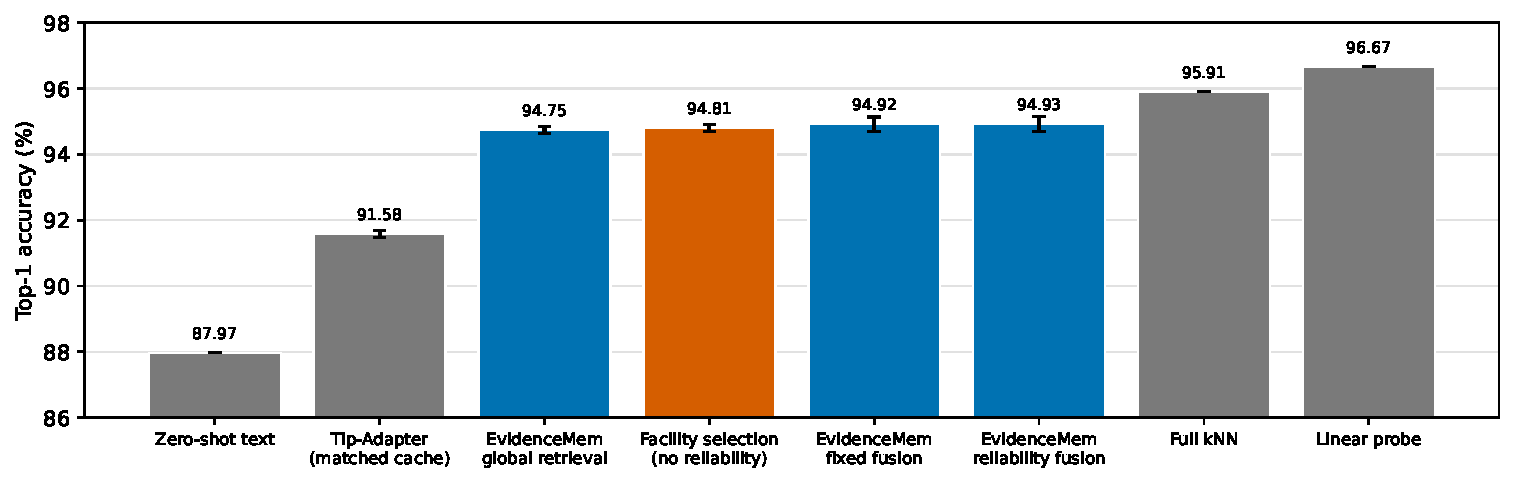
\includegraphics[width=0.93\textwidth]{figures/main_accuracy.pdf}
  \caption{Confirmatory top-1 accuracy on the frozen 3,300-image split. Bars summarize
  five memory seeds where a method is stochastic. The linear probe and full kNN retain
  an accuracy advantage; \method{} uses 440 stored images rather than the 13,200-image
  kNN support set.}
  \label{fig:main}
\end{figure*}

\section{Related Work}

\paragraph{Frozen vision--language representations.}
CLIP demonstrated that natural-language supervision can produce image representations
that transfer through text-defined classifiers~\cite{radford2021learning}. SigLIP~2
extends this family with a revised training recipe and stronger transfer and localization
behavior~\cite{tschannen2025siglip2}. We use a frozen SigLIP~2 checkpoint as a feature
extractor and do not fine-tune its parameters. The question is therefore about the
external memory and scoring rule, not representation learning.

\paragraph{Cache-based adaptation.}
Tip-Adapter augments text logits with similarities to a labeled feature cache, providing
a training-free few-shot adaptation rule~\cite{zhang2022tipadapter}. ProKeR later
interpreted cache adapters as local kernel methods and argued for incorporating global
information~\cite{bendou2025proker}. \method{} shares the use of a frozen feature space
and a labeled cache, but imposes an exact per-class storage budget and retains source
medoids. We include Tip-Adapter with the same 440-example cache budget. This experiment
does not claim a new state of the art in few-shot adaptation because it covers one
curated dataset and one selected encoder.

\paragraph{Coverage selection.}
Facility-location objectives reward a set whose members are similar to the remaining
data. With nonnegative similarities, the usual maximum-coverage form is monotone and
submodular, and cardinality-constrained greedy maximization has the standard
approximation result~\cite{nemhauser1978analysis}. That property concerns coverage of
the frozen embedding set; it is not an accuracy guarantee. In our confirmatory method,
facility coverage determines the stored support set and reliability changes only its
downstream scores.

\section{Method}
\label{sec:method}

\subsection{Task and frozen representations}

Let $\mathcal{D}=\{(x_i,y_i)\}_{i=1}^{n}$ be a labeled support set with $C$ classes.
A frozen image encoder $f$ produces a unit-normalized vector
$z_i=f(x_i)/\lVert f(x_i)\rVert_2$. A frozen text encoder produces one class vector
$t_c$ by averaging and normalizing six prompted descriptions of class $c$. The memory
budget is $B$ real images per class, so the complete memory contains $BC$ prototype
vectors and their source identifiers.

\subsection{Coverage-selected real-image prototypes}

For each class, we first fit $2B$ mini-batch k-means clusters~\cite{sculley2010web} to
its support vectors. The
candidate for a cluster is the member nearest its normalized centroid, which guarantees
that every candidate maps to a displayable source image. We then greedily select $B$
candidates. If $V_c$ denotes all support vectors in class $c$ and $S_c$ a candidate set,
the selection objective is
\begin{equation}
F_c(S_c)=\frac{1}{|V_c|}\sum_{z\in V_c}\max_{p\in S_c}
\frac{1+z^\top p}{2}.
\label{eq:facility}
\end{equation}
The transform maps cosine similarity to $[0,1]$. Greedy selection starts from an empty
set and adds the candidate with the largest marginal gain until $|S_c|=B$. The same
selected indices are used by the facility control and the reliability-weighted
treatment.

\subsection{Prototype reliability}

Each selected prototype $p_j$ receives three validation-tunable signals. Compactness
$q_j$ is its mean cosine similarity to the members of its original cluster. Purity
$u_j$ is the fraction of its nearest support neighbors that share its label. Text
alignment $a_j=p_j^\top t_{y_j}$ measures agreement with the prompted class vector.
Compactness and text alignment are mapped from $[-1,1]$ to $[0,1]$; purity already lies
on that interval. For nonnegative component weights $w_q,w_u,w_a$, reliability is
\begin{equation}
r_j=\operatorname{clip}\!\left(
\frac{w_q\tilde q_j+w_u u_j+w_a\tilde a_j}{w_q+w_u+w_a},
0.05,1\right).
\label{eq:reliability}
\end{equation}
If an alignment is unavailable, its term is excluded from both numerator and
denominator. The component weights are selected on the validation split for each memory
seed.

\subsection{Class-conditional scoring and fusion}

Global retrieval can exclude a class entirely when its prototypes do not enter the
overall top-$k$. We instead retrieve the $k_c$ most similar prototypes inside every
class. For query vector $z$, class $c$ receives the log-mean-exp score
\begin{equation}
\ell_c^{\mathrm{vis}}(z)=
\log\frac{1}{k_c}\sum_{j\in\mathcal{N}_{k_c}^{c}(z)}
\exp\!\left(\frac{z^\top p_j}{\tau}+\gamma\log r_j\right),
\label{eq:visual}
\end{equation}
where $\tau=0.07$ and $\gamma\geq0$ controls reliability weighting. A softmax across
classes gives $P_{\mathrm{vis}}(y\mid z)$. Text probabilities
$P_{\mathrm{text}}(y\mid z)$ come from cosine similarities to the class text vectors.

The selected prototypes also define a query-level reliability $R(z)$: for each class,
we average the reliabilities of its retrieved prototypes, then average those class
values using $P_{\mathrm{vis}}$. After standardizing $R$ with validation statistics, the
text weight is
\begin{equation}
\alpha(z)=\operatorname{clip}(b+s\,\widehat R(z),0,1),
\qquad
P=(1-\alpha)P_{\mathrm{vis}}+\alpha P_{\mathrm{text}}.
\label{eq:fusion}
\end{equation}
The validation search chooses $w_q,w_u,w_a$, $k_c$, $\gamma$, $b$, and $s$. A final
temperature is also selected on validation negative log likelihood. Four of five seeds
selected $s=0$; the adaptive gate therefore collapsed to a constant in most runs. We
report this because it limits the evidence for query-adaptive fusion.

\subsection{Inference cost and inspectability}

Full kNN compares each query with all $n$ support vectors, which requires
$O(nd)$ similarity work for embedding dimension $d$. The bounded memory compares a
query with $BC$ prototype vectors and therefore requires $O(BCd)$ work. At the default
setting, $n=13{,}200$ and $BC=440$, so the visual search contains 30 times fewer stored
vectors. Prototype construction is an offline cost. It combines class-wise
MiniBatchKMeans with greedy facility selection; neither operation runs when the model
answers a query.

The classifier retains the source identifier for every medoid. A prediction can
therefore return its highest-scoring real images together with the class probability.
This property gives an auditor a concrete record of the retrieved support. It does not
make the retrieved images a causal explanation, and we do not evaluate human trust or
evidence usefulness in this study.

\section{Confirmatory Protocol}
\label{sec:protocol}

\subsection{Data and splits}

The source is the Kaggle collection \emph{130k Images 512x512 Universal Image
Embeddings}.\footnote{\url{https://www.kaggle.com/datasets/rhtsingh/130k-images-512x512-universal-image-embeddings}}
We use the image files, not precomputed third-party embeddings. The 11 categories are
apparel, artwork, cars, dishes, furniture, illustrations, landmark, meme, packaged
products, storefronts, and toys. Sampling is balanced: each class contributes 1,200
training, 200 validation, 300 development, and 300 confirmatory images, for 22,000
retained images. Before the split, SHA-256 and perceptual hashes remove four exact,
four within-label perceptual, and two cross-label perceptual duplicates from the sampled
candidate pool. The split manifest fixes every source path and content hash.

All source files are 512 by 512 pixels. The selected checkpoint,
\texttt{google/siglip2-base-patch16-384}, processes them at 384 by 384 pixels using its
native preprocessing. We use ``512-pixel source images'' and ``384-pixel encoder input''
throughout; treating this experiment as a native 512-pixel encoder comparison would be
incorrect.

\subsection{Freeze and baselines}

Development results fixed sample seed 2026, memory seeds
$\{7,17,29,43,61\}$, the SigLIP~2 checkpoint, the continuous-fusion variant, and
$B=40$. A dedicated confirmatory notebook permits no environment override for the
encoder or evaluation split and checks the frozen repository tag and package tree
before evaluation. No setting was changed after the confirmatory results were read.

The context baselines are full similarity-weighted kNN, an $\ell_2$-regularized linear
probe, and zero-shot text classification. The bounded-memory baselines are random
memory, K-means medoids, and equal-count facility selection. We also include Tip-Adapter
with an equal-count random cache. Full kNN selects $k$ from $\{3,5,10,20\}$ on validation
and chooses $k=10$. The linear probe selects $C$ from $\{0.01,0.1,1,10\}$ and chooses
10. All methods use the same frozen embeddings and data partitions.

\subsection{Hypotheses and uncertainty}

The primary hypothesis is that \method{} at $B=40$ is non-inferior to full kNN with a
margin of one accuracy point. Its decision rule requires the lower end of a hierarchical
paired 95\% interval to exceed $-1$ point. The bootstrap resamples seeds and then examples
within a seed for 5,000 draws. The secondary hypothesis requires the lower end of the
same type of interval for \method{} minus facility selection to exceed zero. We also
report a two-sided exact sign-flip result across the five seed-level differences. With
five seeds, its smallest possible two-sided value is 0.0625, so it is supporting rather
than decisive evidence.

Accuracy and macro F1 summarize classification. We report 15-bin expected calibration
error (ECE) after validation-only temperature selection~\cite{guo2017calibration} and
area under the selective risk--coverage curve (AURC)~\cite{geifman2017selective}.
Reported query time covers the memory or classifier scoring stage only; it excludes
image decoding, preprocessing, and encoder inference.

\subsection{Reproducibility checks}

The run completed on one Tesla T4 with Python 3.12.13 and PyTorch 2.10.0. Its executed
notebook contains 23 cells, including 14 code cells with execution counts 1 through 14
and no error output. The published archive contains 91 unique members and passes a full
CRC check. An independent script checks all 23 files named by the original run manifest,
then loads 65 raw prediction packets. Each packet contains 3,300 labels, predictions,
probabilities, and scores. Recomputed accuracy, balanced accuracy, macro F1, negative
log likelihood, Brier score, ECE, and AURC match the CSV rows to a maximum absolute
difference of $2.22\times10^{-16}$.

\section{Results}
\label{sec:results}

\subsection{Main comparison}

Table~\ref{tab:main} shows the frozen confirmatory result. The linear probe is strongest
at $96.67\%$, followed by full kNN at $95.91\%$. \method{} reaches $94.93\%$ while
retaining 440 images, or one thirtieth of the kNN support set. It improves substantially
over random memory and the matched Tip-Adapter implementation, but those comparisons do
not rescue either predeclared hypothesis.

\begin{table*}[t]
\centering
\small
\caption{Confirmatory classification at the default budget. Values are percentages;
$\pm$ is the standard deviation across five memory seeds. Deterministic baselines have
zero seed variation. ECE is reported after validation-only temperature scaling.}
\label{tab:main}
\begin{tabular}{lrrrr}
\toprule
Method & Stored images & Accuracy & Macro F1 & ECE \\
\midrule
Linear probe & -- & 96.67 & 96.66 & 1.18 \\
Full kNN & 13,200 & 95.91 & 95.88 & 1.20 \\
\method{} reliability-weighted fusion & 440 & $94.93\pm0.22$ & $94.88\pm0.21$ & 1.81 \\
Facility selection, no reliability & 440 & $94.81\pm0.10$ & $94.76\pm0.10$ & 1.87 \\
K-means medoids & 440 & $94.53\pm0.19$ & $94.46\pm0.19$ & 2.54 \\
Random memory & 440 & $92.77\pm0.33$ & $92.67\pm0.33$ & 3.37 \\
Tip-Adapter, matched cache & 440 & $91.58\pm0.11$ & $91.38\pm0.13$ & 4.10 \\
Zero-shot text classifier & 0 & 87.97 & 87.69 & 32.49 \\
\bottomrule
\end{tabular}
\end{table*}

\subsection{Predeclared decisions}

The full-kNN difference is $-0.9818$ points, which lies just inside the one-point margin
as a point estimate. The lower confidence bound is $-1.285$ points, however, so the
required decision rule fails. This is not proof that the method is worse by more than
one point; the interval spans the boundary. It is evidence that this experiment does
not establish non-inferiority.

Against equal-count facility selection, the mean difference is $+0.1212$ points and
the interval includes zero. Seed differences are $+0.303$, $+0.061$, $-0.091$,
$+0.364$, and $-0.030$ points. The reliability treatment therefore has a small and
inconsistent effect. Table~\ref{tab:hypotheses} records both decisions.

\begin{table}[t]
\centering
\small
\caption{Frozen hypothesis tests. Intervals and deltas are accuracy points.}
\label{tab:hypotheses}
\begin{tabular}{lrrr}
\toprule
Comparison & Delta & 95\% interval & Decision \\
\midrule
vs. full kNN & $-0.982$ & $[-1.285,-0.679]$ & Not supported \\
vs. facility & $+0.121$ & $[-0.103,+0.352]$ & Not supported \\
\bottomrule
\end{tabular}
\end{table}

\subsection{Memory budget}

Figure~\ref{fig:budget} and Table~\ref{tab:budget} show the predeclared budget curve.
Accuracy rises monotonically from 20 to 80 prototypes per class. At 80 per class,
\method{} reaches $95.44\%$ with a 15-fold smaller support set than full kNN. Facility
selection reaches $95.53\%$ at the same budget, so the reliability treatment does not
dominate as memory grows. These budget comparisons are exploratory because $B=40$ was
the frozen hypothesis setting.

\begin{figure}[t]
  \centering
  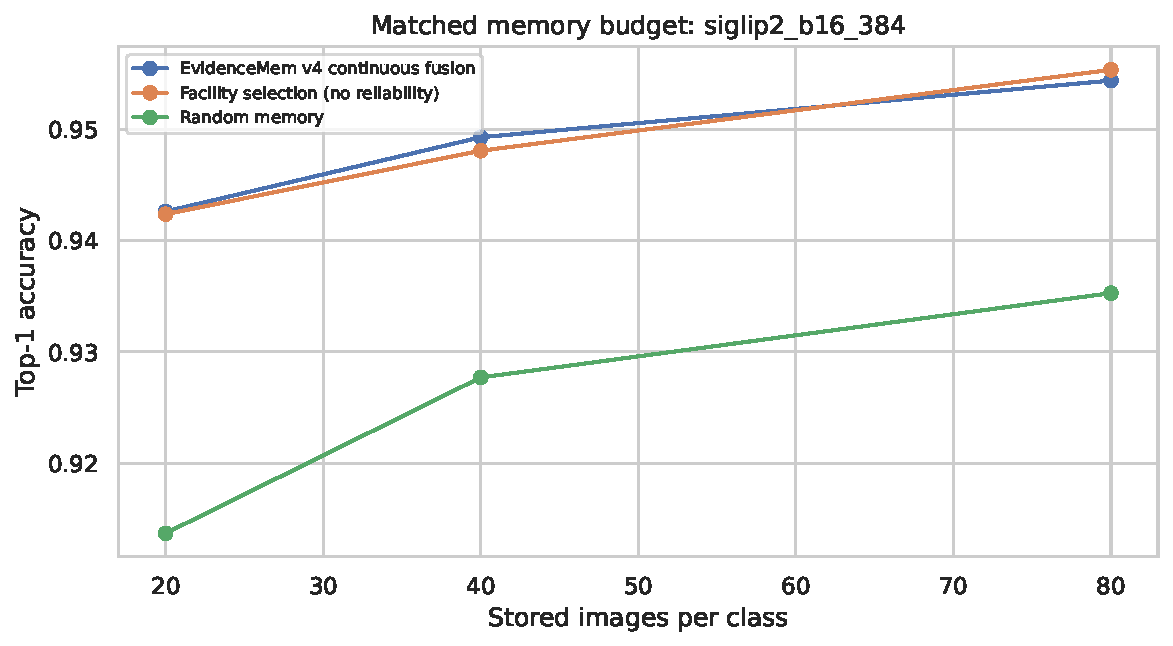
\includegraphics[width=\columnwidth]{figures/memory_budget_accuracy.pdf}
  \caption{Accuracy versus stored images per class. The 20- and 80-image settings are
  exploratory; only 40 per class was used for the frozen primary decision.}
  \label{fig:budget}
\end{figure}

\begin{table}[t]
\centering
\small
\caption{Exploratory budget curve. Accuracy is mean $\pm$ standard deviation across
five seeds; compression is relative to 13,200 training images.}
\label{tab:budget}
\begin{tabular}{rrrr}
\toprule
$B$/class & Stored & Compression & Accuracy \\
\midrule
20 & 220 & $60\times$ & $94.26\pm0.14$ \\
40 & 440 & $30\times$ & $94.93\pm0.22$ \\
80 & 880 & $15\times$ & $95.44\pm0.17$ \\
\bottomrule
\end{tabular}
\end{table}

\subsection{Where compression loses accuracy}

The kNN gap is not uniform across categories. Averaged across memory seeds, artwork is
$5.00$ points below full kNN, illustrations is $2.13$ points below, and storefronts is
$1.00$ point below. Apparel and meme are the only categories where \method{} exceeds
full kNN, by $0.20$ and $0.67$ points. Across the five seed-specific prediction files,
the most frequent \method{} error is artwork predicted as illustrations (132 cases),
followed by artwork as landmark (89) and artwork as meme (51). These labels mix visual
style and semantic content, which makes a small class-balanced memory particularly
sensitive to boundary examples.

The mechanism ablation is equally informative. Class-conditional visual scoring alone
reaches $94.90\%$; fixed fusion reaches $94.92\%$; continuous fusion reaches $94.93\%$.
The three values differ by at most $0.03$ points. Four validation runs set the continuous
gate slope to zero, and three set its intercept to zero. The present evidence therefore
points to class-conditional coverage as the useful part of the tested method, not a
from per-query fusion adaptation.

\subsection{Earlier small-benchmark results}

Table~\ref{tab:precursor} reports the historical classification runs described in
Appendix~\ref{sec:precursor-protocol}. On CIFAR-10, the fused memory reached
$89.58\%$ accuracy with 200 stored prototypes. It exceeded zero-shot CLIP by 4.33
points and K-means medoids by 3.48 points, but remained 4.26 points below the linear
probe. On CIFAR-100, the memory reached $66.73\%$ with 2,000 prototypes. It exceeded
zero-shot CLIP by 3.55 points and remained 8.12 points below the linear probe.

\begin{table*}[t]
\centering
\small
\caption{Exploratory classification on the earlier small-image benchmarks. The fused
memory and K-means values are mean $\pm$ standard deviation over three memory seeds.
These historical runs use a different method and encoder configuration from the
confirmatory study; they provide context, not additional confirmatory evidence.}
\label{tab:precursor}
\begin{tabular}{lrrrrrrr}
\toprule
Dataset & Classes & Stored & Zero-shot & Full kNN & K-means & Fused memory & Linear probe \\
\midrule
CIFAR-10 & 10 & 200 & 85.25 & 82.29 & $86.09\pm0.43$ & $89.58\pm0.11$ & 93.84 \\
CIFAR-100 & 100 & 2,000 & 63.18 & 46.03 & $49.65\pm4.17$ & $66.73\pm0.20$ & 74.85 \\
\bottomrule
\end{tabular}
\end{table*}

The OOD experiment treats CIFAR-10 as in-distribution. Maximum softmax probability
from the fused memory obtains AUROC 0.897 on CIFAR-100 and 0.985 on SVHN. Predictive
entropy performs better, with AUROC 0.907 and 0.991, respectively. At a threshold that
accepts 95\% of CIFAR-10 validation examples, its false-positive rate is 0.520 on
CIFAR-100 and 0.011 on SVHN. The near-OOD result remains difficult. More important,
the proposed disagreement score does not beat predictive entropy. These observations
prevent an unsupported claim that memory-specific confidence improves OOD detection.

The two classification studies also expose a change in representation geometry. Full
kNN trails zero-shot classification on both resized CIFAR datasets but is strong on the
11-category image collection. A compact memory is therefore not uniformly useful
because it is small. Its behavior depends on the encoder, image resolution, class
semantics, and local neighborhood quality. This finding motivated the stronger frozen
protocol and the matched facility control.

\subsection{Calibration and scoring cost}

After validation-only temperature scaling, \method{} has ECE $1.81\%$, close to the
facility baseline's $1.87\%$ but above full kNN's $1.20\%$. Its AURC is 0.00457, compared
with 0.00768 for facility selection and 0.01082 for full kNN. This selective-ranking
result is secondary and should be confirmed on another dataset before it is treated as
a reliability claim.

The measured scoring stage takes 0.060 ms per query for \method{}, 0.018 ms for facility
selection, and 0.103 ms for full kNN. Class-conditional retrieval is slower than a
single search over the same 440 prototypes, yet still faster than the 13,200-vector kNN
search in this implementation. These timings exclude the frozen encoder and were taken
inside one Kaggle run, so they describe the experiment rather than deployment latency.

\subsection{What the evaluation establishes}

The evidence supports three statements. First, the selected real-image memory offers
a measured accuracy--storage tradeoff: it retains 3.33\% of the kNN support images and
loses 0.982 accuracy points on average. Second, coverage selection is consistently
stronger than random storage at the same budget. Third, reliability-aware scoring does
not produce a stable improvement over the matched support set. The evaluation does not
establish accuracy parity, native 512-pixel encoding gains, causal explanations, or
generalization across encoder families. These boundaries define the paper's claims.

\section{Discussion}

The result supports a narrow conclusion. Real-image medoids preserve most of full-kNN
accuracy while reducing the number of stored support images by a factor of 30. That is
a useful operating point for systems that value inspectable examples or bounded storage.
It is not enough to call the method non-inferior under the frozen one-point rule. The
lower confidence bound misses the boundary by 0.285 points.

The reliability mechanism also needs revision. Validation chooses different reliability
components across seeds, and the continuous gate usually becomes constant. Reliability
scores may still help rank evidence. However, the confirmatory comparison does not show
a stable accuracy gain over the same coverage-selected support set. The next experiment
should compare class-conditional scoring with and without reliability power. It should
keep fusion fixed and register the factorial ablation on a new dataset. The current
confirmatory split must remain closed to further tuning.

The linear probe result is another useful boundary. If prediction accuracy is the only
goal and storing model parameters is acceptable, a supervised linear head is better on
this dataset. Prototype memory serves a different need: bounded collections of source
examples that can be retrieved and inspected. A paper about this system should evaluate
that operational value directly, perhaps through evidence fidelity or a human error-audit
study, rather than treating retrieved neighbors as causal explanations.

The precursor results sharpen that conclusion. They show that memory-plus-text fusion
can outperform its visual and textual endpoints on small benchmarks, yet that pattern
does not isolate the source of the gain. The confirmatory controls show that most of the
useful behavior comes from class-conditional coverage. Future work should keep the
support set fixed while testing each scoring component. It should also report a
compute-matched nonparametric baseline and an embedding-only storage comparison.

\section{Limitations}

The experiment uses one selected encoder and one balanced 11-class subset. Encoder
selection occurred on development data, but broader claims need another encoder family
and an external dataset. The source categories are heterogeneous and partly stylistic;
we did not independently relabel the full 22,000-image manifest. Source images are
512 by 512 pixels, while the encoder consumes 384-pixel inputs, so the study does not
measure the effect of native 512-pixel encoding.

The storage comparison counts retained source images, not serialized bytes. A linear
probe and an embedding-only index have different storage and privacy properties, which
image count alone does not capture. Timing excludes encoder inference and is not a
hardware-normalized benchmark. Tip-Adapter was reproduced within the common notebook
rather than run from its authors' repository, although the equation and memory count are
matched.

Only five stochastic seeds are available. The hierarchical bootstrap uses example-level
pairing, while the exact seed-level test has low resolution. Budget results outside
40 images per class are exploratory. Finally, nearest prototypes are associative
evidence. They can expose what the classifier retrieved, but they do not prove why a
prediction was made or whether a visual feature is causally responsible.

The CIFAR and SVHN findings are historical observations, not a second confirmatory
study. Their encoder initialization emitted an activation-mismatch warning, their
selection rule predates the matched-support design, and their result bundle lacks the
complete integrity manifest used for the 22,000-image experiment. We report those
numbers with this qualification instead of silently discarding them. A new registered
run is required before they can support cross-dataset claims about the final method.

\section{Broader Impact}

Bounded memory can reduce the amount of source data retained by an adaptive visual
system, but it does not remove privacy, copyright, or consent concerns. The prototypes
are deliberately recoverable images; that improves inspection and also makes improper
retention visible. Deployments should apply source licensing rules, access controls,
deletion procedures, and class-level audits before treating the memory as a durable
knowledge store.

Reliability and confidence values can be mistaken for guarantees. Our negative
confirmatory result is a reminder that a plausible reliability score may not improve
decisions consistently. High-impact applications should not use this prototype as an
autonomous decision maker. They need domain-specific validation, calibrated escalation
rules, and a way for people to inspect and challenge both the prediction and the stored
evidence.

\section{Conclusion}

We tested a reliability-weighted, class-conditional prototype memory under a frozen
confirmatory protocol. The 440-image memory achieved $94.93\%$ accuracy and a 30-fold
reduction in stored support images relative to full kNN. Its point estimate was within
one percentage point, but the predeclared confidence-bound rule did not establish
non-inferiority. Reliability-aware scoring also failed to show a clear advantage over
equal-count facility selection. The release preserves both outcomes, along with the
executed notebook and raw predictions. The next study should test a simpler, registered
scoring ablation on genuinely new data rather than tune this split again.

\bibliographystyle{plainnat}
\bibliography{references}

\appendix
\section{Prompt Ensemble}

For each class label, the text encoder averages these six templates:
\begin{itemize}
  \item ``a photo whose main category is \{class\}.''
  \item ``a catalog image of \{class\}.''
  \item ``a real-world image showing \{class\} as the main subject.''
  \item ``a wide-view image categorized as \{class\}.''
  \item ``an online image whose visual domain is \{class\}.''
  \item ``an image of \{class\}, not merely a small foreground object.''
\end{itemize}
Class names are expanded where needed. Examples include ``clothing or fashion apparel''
and ``a packaged retail product.'' The exact strings are stored in the notebook source.

\section{Frozen Hyperparameter Search}

The class-specific retrieval grid is $k_c\in\{1,3,5,10\}$. Reliability powers are
$\{0,0.5,1,2\}$. Fixed text weights and continuous intercepts are
$\{0,0.25,0.5,0.75,1\}$. Gate slopes are
$\{-0.5,-0.25,0,0.25,0.5\}$. Reliability component candidates include each individual
component and all pairwise equal mixtures. The grid also includes
$(0.35,0.40,0.25)$ and $(0.45,0.35,0.20)$. Temperature is selected from
$\{0.02,0.03,0.05,0.07,0.10,0.15,0.20,0.50,1\}$. Selection uses validation accuracy
with deterministic tie breaks. The release records the choice for each seed in
\texttt{selected\_hyperparameters.json}.

\section{Reproducibility Map}

The result directory contains the executed notebook, the source-run ZIP, the frozen
protocol, split manifest, classification and budget tables, hypothesis decisions,
figures, per-class analysis, and a release-level SHA-256 manifest. The verification
command is:
\begin{verbatim}
python scripts/verify_confirmatory_release.py
\end{verbatim}
The command checks archive CRCs and hashes, every published file, notebook execution,
prediction shapes and probabilities, and all recomputable classification metrics.

\subsection{Exploratory precursor studies}
\label{sec:precursor-protocol}

Before the confirmatory study, we tested the memory idea on CIFAR-10 and
CIFAR-100~\cite{krizhevsky2009learning}. Both runs used 45,000 training, 5,000
validation, and 10,000 test images resized from 32 pixels to a 224-pixel OpenCLIP
ViT-B/32 input, with three seeds and 20 prototypes per class. CIFAR-100 and
SVHN~\cite{netzer2011reading} also served as OOD inputs for the CIFAR-10 classifier.

These runs use reliability during selection and global fusion, whereas the confirmatory
method uses matched coverage selection and class-conditional scoring. They also record
a noncanonical CLIP activation warning. The results explain the research path but do
not enter the confirmatory statistics or hypothesis decisions.

\section{Confirmatory Error Audit}

Table~\ref{tab:per-class} reports the seed-averaged class results. The compact memory
matches full kNN most closely on apparel and furniture and exceeds it on memes. Its
largest shortfalls occur on artwork and illustrations. These categories are defined
partly by visual style rather than by a single object type, which makes a local
neighborhood sensitive to the boundary between the two labels. The matched facility
control has almost the same class profile. This agreement is consistent with the main
ablation: support-set coverage explains more of the result than the learned reliability
weights.

\begin{table}[t]
\centering
\caption{Confirmatory accuracy by class, averaged over five seeds. All values are
percent. $\Delta$ is \method{} minus full kNN.}
\label{tab:per-class}
\scriptsize
\setlength{\tabcolsep}{3.0pt}
\begin{tabular}{lrrrr}
\toprule
Class & \method{} & kNN & Facility & $\Delta$ \\
\midrule
Apparel        & 99.20 & 99.00 & 99.27 &  0.20 \\
Artwork        & 78.67 & 83.67 & 78.73 & -5.00 \\
Cars           & 99.87 &100.00 & 99.93 & -0.13 \\
Dishes         & 98.73 & 99.67 & 98.20 & -0.93 \\
Furniture      & 97.93 & 98.00 & 97.93 & -0.07 \\
Illustrations  & 93.20 & 95.33 & 93.33 & -2.13 \\
Landmarks      & 95.87 & 96.67 & 96.07 & -0.80 \\
Memes          & 95.67 & 95.00 & 95.80 &  0.67 \\
Packaged goods & 97.67 & 98.33 & 97.53 & -0.67 \\
Storefronts    & 91.67 & 92.67 & 90.73 & -1.00 \\
Toys           & 95.73 & 96.67 & 95.33 & -0.93 \\
\bottomrule
\end{tabular}
\end{table}

Across the five confirmatory predictions, artwork is assigned to illustrations 132
times, to landmarks 89 times, and to memes 51 times; the reverse artwork--illustration
error occurs 39 times. Other recurring pairs include storefronts to illustrations (35),
landmarks to storefronts (32), and memes to illustrations (32). This asymmetry suggests
that the broad artwork class contains modes represented more tightly by neighboring
style or scene classes. More memory may therefore have diminishing returns unless
selection also protects minority modes.

\subsection{Qualitative evidence protocol}

The qualitative release contains six fixed seed-7 queries: three high-confidence errors
and three low-confidence correct predictions. For each query it shows the three
highest-scoring prototypes from the predicted class, their similarities, the text
weight, and reliability. Two errors map artwork to illustrations; one maps artwork to
storefronts. This display supports error inspection, not causal explanation. Because
retrieval is class-conditional, all shown neighbors have the predicted label by
construction. A follow-up study should compare predicted and runner-up evidence and
test counterfactual prototype removal on an unchanged support set.

\end{document}
